\subsection{漸進進化説}
以上で見た進化ゲームは,どのような突然変異も許して議論していた.
つまり,進化の過程は不連続に進みうると考えていた.
この考え方が間違っているわけではない\footnote{「基本的に進化は不連続に進む」という考え方を断続平衡説という.}が,その一方で漸進進化説という考え方もある.
こちらでは,効果の小さい突然変異が積み重なることで生物は連続的に進化すると考える.
漸進進化説では突然変異の可能性が制限されるので,ESSはこれまで「すべての」突然変異に耐性のある戦略と考えてきたが,もっと定義を緩くして,「ありうる」突然変異にだけ耐性があるとしても良さそうである.
また,たとえESSが存在したとしても,生物集団が実際にそこに向かって変異し続けられるとは限らない.
つまり新しく,進化の「収束性」に関わる指標が求められる.
そこで,以降では漸進進化説を採用したときの適応ダイナミクスを考える\footnote{この節での主張は参考文献\cite{text},\cite{jsmb}にあったものだが,先ほどの議論と整合するように文字や関数の定義を若干変更した.また参考文献\cite{text}では省略されていた,ESSと収束安定戦略の定義に至るまでの議論を明記した.}.

\subsection{漸進進化の定式化}
漸進進化の場合でも,式\eqref{fpfq}を導くまでの議論は同じである.
ただし,ここでは野生型と変異型の戦略$p,q$が連続的なパラメータで表せる場合を考える.
ここではごく簡単に,一般に戦略を表す確率分布$r$に対して実数$x(r)$が一対一対応すると仮定し,実数$x(r)$の変動が十分微小となる変異だけが起こりうると考える\footnote{選択肢($S$の元)が$m$個ある場合を考えると,戦略の集合は$\mathbb{R}^{m}$のうち(確率分布として)規格化条件と非負性を満たす部分集合である.たとえば$m=3$なら戦略の集合は$(1,0,0),(0,1,0),(0,0,1)$の3点を結ぶ直線に囲まれた正三角形と対応づけられる.したがって$m=2$の場合を除き,実数に対応づけられる戦略はありうる全戦略の一部にすぎない.つまりここでは,変異だけでなく生物のとりうる戦略自体も限定して考えている.}.
その仮定の下で野生型と変異型の戦略をそれぞれ
\begin{equation}
  x \coloneqq x(p),\qquad x' \coloneqq x(q)
\end{equation}
と実数で表し,これを用いて
\begin{align}
  F(x,x) \coloneqq F(p,p),\qquad &F(x,x') \coloneqq F(p,q), \\
  F(x',x) \coloneqq F(q,p),\qquad &F(x',x') \coloneqq F(q,q)
\end{align}
と書くことにする.
このとき,式\eqref{fpfq}は
\begin{equation}
  F_{x} \approx (1-\epsilon)F(x,x) + \epsilon F(x,x') ,\qquad F_{x'} \approx (1-\epsilon)F(x',x) + \epsilon F(x',x') 
\end{equation}
と書ける.
これをもとに,変異型の相対適応度を次のように定義する:
\begin{equation}
  F(x'|x) \coloneqq F_{x'} - F_{x}
\end{equation}
これが正(負)のとき,変異型は野生型を侵入することができる(できない).
また,定義より任意の戦略$x$に対して
\begin{equation}
  F(x|x) = 0 \label{F0}
\end{equation}
が成り立つ.

ここで,ある戦略$x^*$が野生型となった状態を考え,ここに戦略$x^*+\delta$が変異型として現れたとする($\delta$は実数).
このとき定義\ref{ess}をもとにすると,戦略$x^*$がESSとは,変異として可能な任意の$\delta$に対して
\begin{align}
  F(x^*+\delta|x^*) &= F(x^*+\delta | x^*) - F(x^*|x^*) \notag\\
  &= \delta\left.\frac{\partial F(x'|x)}{\partial x'}\right|_{x'=x=x^*} + \frac{\delta^2}{2}\left.\frac{\partial^2 F(x'|x)}{\partial x'^2}\right|_{x'=x=x^*} + \order{\delta^3} < 0 \label{ess1}
\end{align}
が成り立つことであるといえそうである.
ここで$\delta_0$をある微小な正数とし,$\delta$が$-\delta_0 < \delta < \delta_0$の範囲にあるような変異が許されると考える.
つまりこの範囲にある任意の$\delta$について上式が成り立つとする.
このとき,上式を$\lvert \delta \rvert$で割って$\delta \to \pm 0$それぞれの極限をとると,$\delta/\lvert\delta\rvert \to \pm 1$に注意して,
\begin{equation}
  \pm \left.\frac{\partial F(x'|x)}{\partial x'}\right|_{x'=x=x^*} \le 0 
\end{equation}
がいえる.
これがどちらの極限をとっても成り立つので,
\begin{equation}
  \left.\frac{\partial F(x'|x)}{\partial x'}\right|_{x'=x=x^*} = 0
\end{equation}
となる.
また,式\eqref{ess1}を$\delta^2$で割って$\delta \to 0$の極限をとると,今度は
\begin{equation}
  \frac{1}{2}\left.\frac{\partial^2 F(x'|x)}{\partial x'^2}\right|_{x'=x=x^*} \le 0
\end{equation}
が得られる.
ただしここで等号が成り立つとき,ESSの判定にさらに高次の項の情報が必要となって不便である.
そこでESSを次のように定義する.
\begin{dfn}[漸進進化における進化的安定戦略]
  戦略$x^*$が進化的安定戦略(ESS)であるとは,
  \begin{equation}
    \left.\frac{\partial F(x'|x)}{\partial x'}\right|_{x'=x=x^*}=0 ,\qquad \left.\frac{\partial^2 F(x'|x)}{\partial x'^2}\right|_{x'=x=x^*} < 0 
  \end{equation}
  が成り立つことである.
\end{dfn}

次に収束安定性を議論する.
戦略$x^*$が収束安定戦略であるとは,その戦略$x^*$に近い戦略をとる野生型がもっと$x^*$に近い変異型に置き換わることである.
つまり,野生型が$x^*$に十分近い戦略$x$をとるとき,$x$よりも戦略$x^*$に近い戦略$x'$をとる変異型に侵略されるということである.
そこで$x-x^*=\delta,\, x'-x=\delta'$とおくと,これは$\delta$と$\delta'$が異符号のとき$F(x'|x)>0$,$\delta$と$\delta'$が同符号のとき$F(x'|x)<0$と言い換えられる.
つまり次が成り立つ:
\begin{equation}
  \delta \delta' F(x'|x) < 0
\end{equation}
そこでこの左辺を変形すると,
\begin{align}
  \delta \delta' f(x'|x) &= \delta \delta' f(x + \delta'|x) = \delta \delta' \qty{f(x+\delta'|x) - f(x|x)}\notag\\ 
  &= \delta \delta' \qty{\delta'\left.\frac{\partial F(x'|x)}{\partial x'}\right|_{x'=x} + \order{\delta'^2}} = \delta \delta'^2 \left.\frac{\partial F(x'|x)}{\partial x'}\right|_{x'=x=x^*+\delta} + \order{\delta'^3} \notag\\
  &= \delta \delta'^2 \qty{\left.\frac{\partial F(x'|x)}{\partial x'}\right|_{x'=x=x^*} + \delta \left.\frac{\partial}{\partial x}\qty(\left.\frac{\partial F(x'|x)}{\partial x'}\right|_{x'=x}) \right|_{x=x^*}+\order{\delta'^2}} + \order{\delta^3} \notag \\
  &= \delta\delta'^2 \left.\frac{\partial F(x'|x)}{\partial x'}\right|_{x'=x=x^*} + \delta^2\delta'^2 \left.\frac{\partial}{\partial x}\qty(\left.\frac{\partial F(x'|x)}{\partial x'}\right|_{x'=x}) \right|_{x=x^*} + \order{\delta^3, \delta'^3}
\end{align}
となる.
この式についてESSのときと同様に極限を考えれば,収束安定戦略を次のように定義すれば良いことが分かる.
\begin{dfn}[収束安定戦略]
  戦略$x^*$が収束安定戦略(convergence stable strategy\footnote{後述する連続安定戦略と重複するため,ここではCSSとは略さない.})であるとは,
  \begin{equation}
    \left.\frac{\partial F(x'|x)}{\partial x'}\right|_{x'=x=x^*} = 0 ,\qquad
    \left.\frac{\partial}{\partial x}\qty(\left.\frac{\partial F(x'|x)}{\partial x'}\right|_{x'=x}) \right|_{x=x^*} < 0
  \end{equation}
  が成り立つことである.
\end{dfn}

また,ESSと収束安定戦略の定義を見比べると,両方とも
\begin{equation}
  \left.\frac{\partial F(x'|x)}{\partial x'}\right|_{x'=x=x^*} = 0
\end{equation}
が含まれる.
これが成り立つような戦略$x^*$は進化の到達点の候補であり,進化的特異点と呼ばれる.

\subsection{PIPによる可視化}
これまで,1つのパラメータで記述できる漸進進化の適応ダイナミクスについてESSと収束安定戦略を定義した.
ここではこの適応ダイナミクスを可視化し,集団内の戦略の遷移をより直観的に捉える手法を紹介する.

まず横軸に野生型の戦略$x$をとり,縦軸に変異型の戦略$x'$をとる.
次にこの2次元平面を,$F(x'|x)$の正負によって塗り分ける.
たとえば$F(x'|x)>0$の領域を黒に,$F(x'|x)<0$の領域を白に塗り分ける.
こうしてできたグラフをPIP(Pair-wise Invasibility Plot)という.
グラフの作り方から,白黒の境目では$F(x'|x)=0$が常に成り立つ.

相対適応度を表す関数$F(x'|x)$によっていろいろなPIPはあり得るが,式\eqref{F0}より,直線$x=x'$は白黒の領域の境目になり得る.
ここでは簡単のため,直線$x=x'$が常に白黒の領域の境目になる状況を考える.
また$x=x'$は変異型が存在しない状態を意味するので,PIPを読み取る上で重要である.
たとえば,最初$x=x'$上にある状態に新しく変異型が生まれ,それが侵入して集団全体に定着すると再び$x=x'$上に戻る.
これを繰り返すような適応ダイナミクスを考えると,直線$x=x'$の近傍における白黒が重要になる.
ここで,もし直線$x=x'$から少し上($+x'$)方向にずれたところが常に黒で,下($-x'$)方向にずれたところでは常に白だとすると,$x$の大きな戦略が次々と侵入し,$x$は無制限に大きくなっていく.
逆に下方向にずれたところで常に黒,上方向にずれたところでは常に白の場合は,$x$は無制限に小さくなっていく.

では,直線$x=x'$上に$F(x'|x)=0$となる別の曲線が交わり,それを境に$x=x'$の上下の状況が変わったらどうなるだろうか.
ここではそれを図\ref{fig:pip}に示した4通りの状況に分けて考える.

\begin{figure}[htbp]
  \centering
  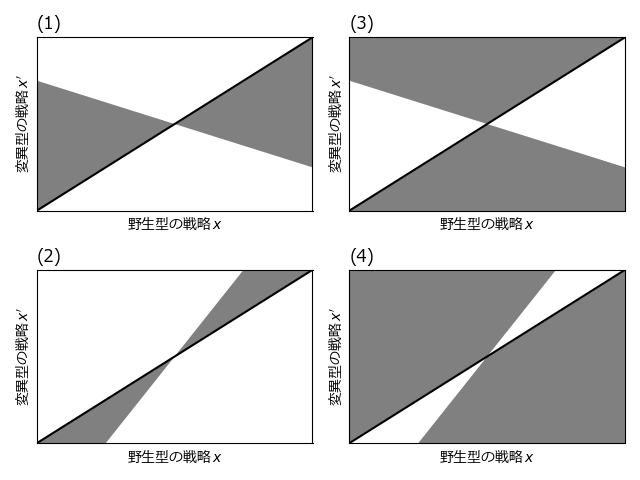
\includegraphics[width=13cm]{pip.png}
  \caption{代表的なPIP.直線$x=x'$は太線で示し,$F(x'|x)>0$の領域を灰色で,$F(x'|x)<0$の領域を白色で塗りつぶした.また2つの直線の交点の座標を$(x^*,x^*)$とする.}
  \label{fig:pip}
\end{figure}

図\ref{fig:pip}(1)の場合,戦略$x<x^*$の野生型は戦略$x'>x$の変異型に侵入され,戦略$x>x^*$の野生型は戦略$x'<x$の変異型に侵入される.
よって戦略$x^*$は収束安定戦略である.
また,$x^*$はその付近の変異型に侵入されないので,ESSでもある.
このような戦略$x^*$は連続安定戦略(continuously stable strategy:CSS)と呼ばれ,適応ダイナミクスにより実現し安定に持続する.

図\ref{fig:pip}(2)の場合,戦略$x<x^*$の野生型は戦略$x'<x$の変異型に侵入され,戦略$x<x^*$の野生型は戦略$x'>x$の変異型に侵入される.
よって戦略$x^*$は収束安定戦略ではない.
また,$x^*$はその付近の変異型に侵入されるので,ESSでもない.
このような戦略$x^*$は,適応ダイナミクスにより実現しない上に持続できない.

図\ref{fig:pip}(3)の場合,戦略$x^*$の収束性は(2)と同じであり,進化的安定性は(1)と同じである.
よって戦略$x^*$は収束安定戦略ではないがESSである.
このような戦略$x^*$は,仮に実現すれば安定に持続するが,適応ダイナミクスで実現することはない.
この状況を旧約聖書になぞらえて,戦略$x^*$をエデンの園と呼ぶこともある.

図\ref{fig:pip}(4)の場合,戦略$x^*$の収束性は(1)と同じであり,進化的安定性は(2)と同じである.
よって戦略$x^*$は収束安定戦略だがESSではない.
このような戦略$x^*$は適応ダイナミクスにより実現するものの,すぐに変異型に侵入されてしまう.
言い換えれば,$x^*$は変異型としては強いが野生型になると弱くなる戦略なのである.
これは先述した単純な「最適化」では記述できなかった状況である.
ところが集団全体が$x^*$になったときに,$x_1>x^*$となる戦略$x_1$と$x_2<x^*$となる戦略$x_2$が同時に出現することもあり得る.
このとき$x_1,x_2$は$x^*$に打ち勝ち,集団内には$x_1$と$x_2$だけが残る.
PIP図を見るとこれらは互いに侵入可能に見えるが,これは$x_1,x_2$のどちらかが大半を占めているときの図なので,両方が同じくらいの頻度のときには使えない.
そこで,この場合に新しく(局所的な)相対適応度を定義し直すと,$x_1,x_2$よりも$x^*$から遠い戦略をとる個体が侵入可能であることが分かる\cite{geritz}.
こうして戦略は$x^*$から離れる方向に二分化する.
(ただしこの相対適応度は局所的なものなので,ある程度$x^*$から離れると侵入がなくなると考えられる.)
実際にこれをもとにしたシミュレーションによって,もともと集団全体が一つの戦略をとっていたとしても二つの戦略に分裂するという現象が確認されている.
このような現象を進化的分岐といい,このような戦略$x^*$を進化的分岐点という.
この進化的分岐は,同一の環境に生息する生物の種分化(同所的種分化)に関連すると考えられている\footnote{分裂した二戦略$x_1,x_2$がそれぞれ「種」として独立するためには,$x_1$をとる個体と$x_2$をとる個体の間の交配に制限がかかることが重要であると考えられている.}.